\documentclass[compress,9pt]{beamer}

%%%%%%% PACKAGES %%%%%%%%%
\usepackage[french]{babel}
\usepackage[backend=biber,style=authoryear,bibstyle=authoryear,natbib=true,
giveninits=true,uniquename=false,uniquelist=false,maxcitenames=2,date=year,
maxbibnames=99,url=false]{biblatex}
\addbibresource{Thèse.bib}
\usepackage{tikz}
\usepackage[T1]{fontenc}
\usepackage[utf8]{inputenc}
\usepackage{amsfonts}
\usepackage{amssymb}
\usepackage{lmodern}
\usepackage[absolute,overlay]{textpos}
\usepackage{contour}
\usepackage{ulem}
\usepackage{xcolor}
\usepackage{newunicodechar}
\usepackage{multirow}
\usepackage{setspace}
\usepackage{pifont}
\usepackage{appendixnumberbeamer}
%\usepackage{animate}

%%%%%%% PARAMETERS %%%%%%%%%
	%%%%%% CITE PARAMETERS %%%%%%%%%%%
		\AtEveryCitekey{\clearfield{title}\clearfield{note}\clearfield{pages}\clearlist{location}					\clearlist{publisher}\clearname{editor}\clearfield{issn}\clearfield{doi}}
		\renewcommand*{\multicitedelim}{\\}
		\renewcommand{\footfullcite}[1]{\footnote[frame]{\fullcite{#1}}}
		\def\bibfont{\tiny}			% Réduit la taille de la police dans les références biblio
	%%%%%% THEME %%%%%%%%
		\usetheme{Madrid}
		\useoutertheme[subsection=false]{miniframes}
		\usefonttheme{structurebold}
		\usepackage{etoolbox}
		\makeatletter
		\patchcmd{\slideentry}{\advance\beamer@xpos by1\relax}{}{}{}
		\def\beamer@subsectionentry#1#2#3#4#5{\advance\beamer@xpos by1\relax}%
		\makeatother
		\definecolor{myblue}{RGB}{143, 174, 217}%{120,150,200}
		\usecolortheme[named=myblue]{structure}
		\beamertemplatenavigationsymbolsempty 
		\setbeamerfont{page number in head/foot}{size=\tiny}
		\setbeamerfont{section in head/foot}{size=\scriptsize}
		\setbeamerfont{section in toc}{size=\footnotesize}
		\setbeamerfont{subsection in toc}{size=\tiny}
		\setbeamerfont{frametitle}{size=\large}
		\setbeamerfont{block title}{size=\normalsize}
		\setbeamerfont{block body}{size=\normalsize}
		\setbeamertemplate{footline}[frame number]
%		\setbeamertemplate{footnote}{size=\tiny}
		\setbeamertemplate{footcite}{site=\tiny}
		\setbeamercovered{transparent}
	%%%% ??
	\newcommand{\cmark}{\ding{51}}
	\newcommand{\xmark}{\ding{55}}
	\newcommand\Wider[2][3em]{%
	\makebox[\linewidth][c]{%
	  \begin{minipage}{\dimexpr\textwidth+#1\relax}
	  \raggedright#2
	  \end{minipage}%
	  }%
	}
	
%%%%%%%% TITLE %%%%%%%%%
\title{Comment valoriser les données anciennes pour l’analyse fréquentielle des crues : application au Rhône à Beaucaire de 1500 à 2020}
\author{Mathieu LUCAS}
\date{3 juillet 2023}

%%%%%%%%% MAIN PART %%%%%%%%%%
\begin{document}

%%%%%% PAGE DE TITRE %%%%%%%%
{
\usebackgroundtemplate{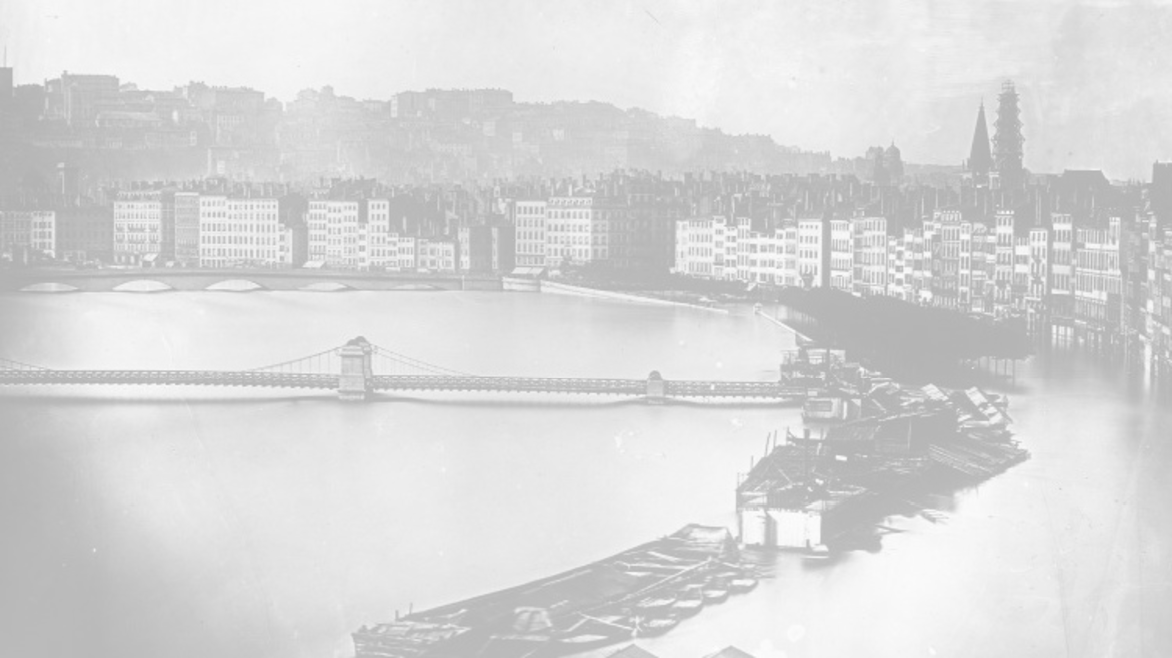
\includegraphics[height=\paperheight,width=\paperwidth]{./Figures/Back.pdf}}

\begin{frame}[plain]
     \vfill
%     
\includegraphics[width= .1\textwidth]{./Figures/CNR.png}  
%     
\includegraphics[width= .1\textwidth]{./Figures/h2o.png}  
%     \includegraphics[width= .1\textwidth]{./Figures/logo_inrae.jpg}  
%     
\includegraphics[width= .1\textwidth]{./Figures/lyon1.png}  
%     
\includegraphics[width= .1\textwidth]{./Figures/MEGA.png}  
     \centering
     \begin{beamercolorbox}[sep=8pt,center,colsep=-4bp,rounded=true,shadow=true]{institute}
     \end{beamercolorbox}
     {\usebeamercolor[fg]{titlegraphic}\inserttitlegraphic\par}
     \begin{beamercolorbox}[sep=12pt,center,colsep=-4bp,rounded=true,shadow=true]{title}
        \usebeamerfont{title}\inserttitle\par%
        \ifx\insertsubtitle\@empty%
        \else%
        \vskip0.25em%
        {\usebeamerfont{subtitle}\usebeamercolor[fg]{subtitle}\insertsubtitle\par}%
      \fi%     
     \end{beamercolorbox}%
     \vskip1em\par
     \begin{beamercolorbox}[sep=12pt,center,colsep=-4bp,rounded=true,shadow=true]{author}
%        \usebeamerfont{author}
        \Large{\insertauthor}
     \end{beamercolorbox}
    \begin{beamercolorbox}[sep=12pt,center,colsep=-4bp,rounded=true,shadow=true]{author}
   
%   \noindent \normalsize Devant le jury composé de :\\
%\vspace{\stretch{1}}
%\begin{adjustwidth}{-0.8cm}{}
\begin{center}
\noindent \scriptsize{
\begin{tabular}{llrl}
    	\textsc{Carreau} & Julie & Professeure adjointe, Université de Montréal & Rapporteure\\
    	\textsc{Llasat} & Maria-Carmen & Professeure, Université de Barcelone & Rapporteure\\
    	\textsc{Favre}	& Anne-Catherine & Professeure, Université Grenoble Alpes & Examinatrice\\
      	\textsc{Payrastre} & Olivier & IDTPE, Université Gustave Eiffel & Examinateur\\
      	\textsc{Riviere} & Nicolas & Professeur, INSA Lyon & Examinateur\\
      	\textsc{Ribereau} & Pierre & Maître de Conférences,  Université Lyon 1 & Examinateur\\
      	\textsc{Lang} & Michel & ITPEHC , INRAE Villeurbanne & Directeur de thèse \\
      	\textsc{Le Coz} & Jérôme & ICPEF, INRAE Villeurbanne & Co-encadrant\\
      	\textsc{Renard} & Benjamin& Chargé de Recherche, INRAE Aix-en-Provence& Co-encadrant\\
      	\textsc{Pierrefeu} & Gilles & Ingénieur, CNR & Invité \\
\end{tabular}
}
\end{center}
%\end{adjustwidth}
   
   
   
   
   
%%    \begin{center}
%	    \begin{columns}[t]
%	    	\begin{column}[t]{0.35\textwidth}
%				\flushright{\small{Encadrement :}}
%			\end{column}%
%			\begin{column}{0.45\textwidth}
%			\begin{flushleft}			
%				\small{Michel LANG (INRAE RiverLy) \newline
%				Jérôme LE COZ (INRAE RiverLy) \newline
%				Benjamin RENARD (INRAE RECOVER)}
%			\end{flushleft}
%			\end{column}%
%			\begin{column}{0.25\textwidth}
%			\end{column}%
%	    \end{columns}
%	\end{center}
	
%    \small{\underline{Encadrement} : Michel LANG (INRAE RiverLy) \newline
%    \textcolor{white}{Encadrement :} Jérôme LE COZ (INRAE RiverLy) \newline
%    \textcolor{white}{Encadrement :    } Benjamin RENARD  (INRAE RECOVER)}
    \end{beamercolorbox}
     \begin{beamercolorbox}[sep=8pt,center,colsep=-4bp,rounded=true,shadow=true]{date}
        \usebeamerfont{date}\insertdate
     \end{beamercolorbox}\vskip0.5em
% 	\vspace*{1cm}


%
%\begin{centering}
%\begin{columns}[b]
%\begin{column}{0.15\textwidth}
%\includegraphics[height=8mm]{./figures/intro/logoUGA.pdf} 
% \end{column}%
% \begin{column}{0.15\textwidth}
%  \textcolor{white}{bla}
% \end{column}
%\begin{column}{0.15\textwidth}
%\includegraphics[height=9mm]{./figures/intro/logoEDF.pdf} 
% \end{column}%
% \begin{column}{0.15\textwidth}
%  \textcolor{white}{bla}
% \end{column}
% \begin{column}{0.15\textwidth}
%\includegraphics[height=4mm]{./figures/intro/logoINRAE.pdf}
% \end{column}
%\end{columns}
%
%\end{centering}

\end{frame} 
}

\section{Introduction}
	\subsection{Le risque de crue}
	
	%%%%%%%%% 2 %%%%%%%%%
	\begin{frame}[c]
		\frametitle{Le risque de crue}
      	\begin{minipage}{0.49\textwidth}

      		\begin{itemize}
      			\item<1->[$\vartriangleright$] Type de catastrophe naturelle le plus fréquent dans le monde au XXI\textsuperscript{ème} siècle\footfullcite{undrr_human_2020}
      			\vspace{10pt}
      			\item<2->[$\vartriangleright$] Plus de 104 000 décès de 2000 à 2019
      		\end{itemize}
      	\end{minipage}
      	\hfill
      	\begin{minipage}{0.49\textwidth}
      		\begin{center}
      			\item \includegraphics<1>[width= .9\textwidth]{./Figures/Crue2005TyrolBBA-Imst.jpg}  
				\item \includegraphics<2>[width= .9\textwidth]{./Figures/UNDRR.png}  
%				\vspace{3pt}    	
%				\item \includegraphics<3>[width = .9\textwidth]{./Figures/UNDRR-2.jpg} 
      		\end{center}
      	\end{minipage}
	\end{frame}
		
	\subsection{L'estimation du risque}
	
	%%%%%%%%% 3 %%%%%%%%%
	\begin{frame}%[c]
		\frametitle{L'estimation du risque}
      	\begin{minipage}{0.5\textwidth}
      		Nécessité de caractériser statistiquement l'aléa de crue :
      		\vspace{10pt}
      		\begin{itemize}
      			\item<2->[$\vartriangleright$] Plan de Prévention du Risque Inondation : \og\textit{déterminé à partir de l'événement le plus important connu ou d'un évènement théorique de \textbf{fréquence centennale}, si ce dernier est plus important}\fg{} \footfullcite{Code de l'environnement; article R562-11-3}
      			\vspace{10pt}
      			\item<4>[$\vartriangleright$] Dimensionnement d'infrastructures à risque (évacuateurs de crue, digues de protection...) : \textbf{périodes de retour jusqu'à 10 000 ans}
      		\end{itemize}
      	\end{minipage}
      	\begin{minipage}{0.45\textwidth}
      		\begin{center}
  
				\item \includegraphics<3>[width = .9\textwidth]{./Figures/PPRI_lyon.pdf}  
				\item \includegraphics<4>[width = .8\textwidth]{./Figures/Grangent.jpg} 
      		\end{center}
      	\end{minipage}
	\end{frame}
	
	%%%%%%%%% 4 %%%%%%%%%
	\begin{frame}%[c]
		\frametitle{Prédétermination des crues}
		Domaine de la \textbf{prédétermination} $\neq$ prévision\\
		\vspace{10pt}
		\onslide<1-> Le débit d'une crue de période de retour $T$
		\vspace{10pt}
      	\begin{itemize}
			\item<2->[$\vartriangleright$] a une probabilité $p = 1/T$ d'être dépassé chaque année
			\vspace{2pt}
			\item<3->[$\vartriangleright$] a une probabilité $p = 1 - 1/T$ de ne pas être dépassé
		\end{itemize}
		\vspace{5pt}
		\centering
		\includegraphics<4->[width = .1\textwidth]{./Figures/Attention.png} 
		\begin{itemize}
			\item<5->[$\vartriangleright$] Une crue centennale n'apparait pas tous les 100 ans
			\item<5->[$\vartriangleright$] On peut observer 2 crues centennales deux années de suite
		\end{itemize}
	\end{frame}
	
	  
	\subsection{Crues et statistiques}
	%%%%%%%%% 5 %%%%%%%%%
	\begin{frame}[t]
		\frametitle{Crues et probabilités}
      	2 grandes familles de méthodes : 
      	\vspace{20pt}
      	\newline
      	\begin{minipage}{0.49\textwidth}
      		\begin{center}
      			\begin{itemize}
      				\item<2->[$\vartriangleright$] Approche basée sur les données de pluie
      			\end{itemize}	
      			\vspace{5pt}
				\includegraphics<2->[width = .92\textwidth]{./Figures/Pluie.jpg} 
			\end{center}
		\end{minipage}
		\begin{minipage}{0.49\textwidth}	
			\begin{center}
				\begin{itemize}
      				\item<3>[$\vartriangleright$] Approche basée sur les données de débit
      			\end{itemize}
      			\vspace{5pt}
				\includegraphics<3>[width = .95\textwidth]{./Figures/EchelleLimni.jpg} 
			\end{center}
		\end{minipage}
	\end{frame}
	
	%%%%%%%%% 6 %%%%%%%%%
	\begin{frame}[c]
		\frametitle{Crues et probabilités}
      	2 grandes familles de méthodes : \newline
		\begin{center}
			\begin{itemize}
				\centering
      			\item[$\vartriangleright$] Approche basée sur les séries de débit
      			\vspace{5pt}
      			\begin{center}
      				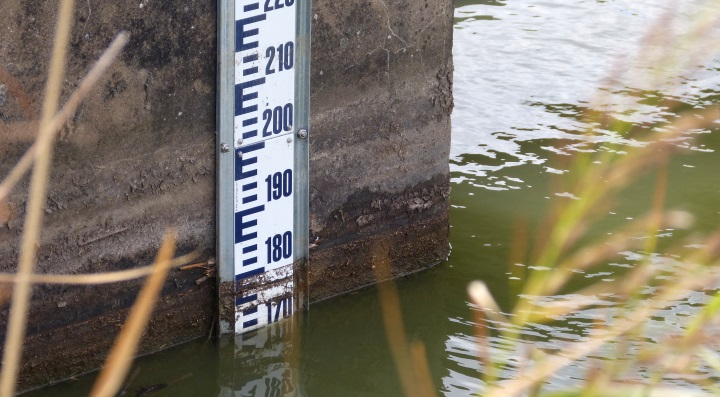
\includegraphics[width = .6\textwidth]{./Figures/EchelleLimni.jpg} 
      			\end{center}	
				\begin{itemize}
					\centering
      				\item<2->[$\checkmark$] \normalsize{Adaptée aux grands bassins versants}
      				\vspace{5pt}
      				\item<3->[$\checkmark$] \normalsize{Adaptée à l'utilisation de données historiques}
      			\end{itemize}		
      		\end{itemize}		
		\end{center}
	\end{frame}
	
		
	%%%%%%%%% 7 %%%%%%%%%    %crues = réalisations + concept de période de retour
	\begin{frame}%[c]
		\frametitle{Analyse fréquentielle des crues}
		L'analyse fréquentielle des crues repose sur les hypothèses suivantes : 
      	\vspace{3pt}			
		\begin{center}
			\includegraphics[width = .8\textwidth]{./Figures/Réalisations.pdf} 
		\end{center}
		\vspace{5pt}
		\begin{itemize}
			\item<2->[$\vartriangleright$] Les observations de crues $(x_1,...,x_n)$ sont des réalisations d'une variable aléatoire $X$ 
			\vspace{5pt}
			\item<3->[$\vartriangleright$] Il est possible de modéliser le comportement de $X$ à l'aide d'une distribution statistique 
		\end{itemize}
		\centering
		\onslide<4->{$\mathcal{Lognormal}(\textcolor{red}{\mu,\sigma^{2}})$ - $Gumbel(\textcolor{red}{\mu,\beta})$ - $GEV(\textcolor{red}{\mu,\sigma,\xi})$}
	\end{frame}

	%%%%%%%%% 8 %%%%%%%%%
	\begin{frame}%[c]
		\frametitle{Analyse fréquentielle des crues}
		\begin{center}
			\includegraphics<1>[width = .8\textwidth]{./Figures/Qamax.pdf} 
			\includegraphics<2>[width = .8\textwidth]{./Figures/Qamax_GEV.pdf} 
			\includegraphics<3>[width = .8\textwidth]{./Figures/Qamax_GEV_Q100.pdf} 
		\end{center}
	\end{frame}
		
	\subsection{Incertitudes}
	%%%%%%%%% 9 %%%%%%%%%
	\begin{frame}%[c]
		\frametitle{Analyse fréquentielle et incertitudes}
		Ces estimations affectées par des incertitudes :
		\vspace{10pt}
      	\begin{itemize}
      		\item<2-7>[$\vartriangleright$] \textbf{Hypothèses de modélisation} : \onslide<3-7>{choix d'une distribution, stationnarité...}
      		\vspace{5pt}
      		\item<4-7>[$\vartriangleright$] \textbf{Données d'entrée} : \onslide<5-7>{estimation indirecte du débit des cours d'eau}
      		\vspace{5pt}
      		\item<6-7>[$\vartriangleright$] \textbf{Échantillonnage} : \onslide<7>{longueur limitée des échantillons de crues}
      	\end{itemize}
      	\vspace{10pt}
      	\centering
      	\onslide<8> Leur détermination est essentielle
	\end{frame}
	
	%%%%%%%%% 10 %%%%%%%%%
	\begin{frame}%[c]
		\frametitle{Incertitudes hydrométriques}
      	\onslide<1-4>\textbf{Le débit des cours d'eau ne peut être mesuré en continu}
      	\begin{itemize}
      		\item<2-4>[$\vartriangleright$] Mesure de la hauteur d'eau
		\end{itemize}
%		\vspace{3pt}
		\begin{center}
			\includegraphics<3>[width = .7\textwidth]{./Figures/LimniVienne.png}
			\includegraphics<4>[width = .7\textwidth]{./Figures/Hydrom1.pdf}
			\includegraphics<5>[width = .7\textwidth]{./Figures/4Jau.pdf}
			\includegraphics<6>[width = .7\textwidth]{./Figures/Hydrom2.pdf}
			\includegraphics<7>[width = .7\textwidth]{./Figures/Hydrom3.pdf}
		\end{center}
	\end{frame}
	
	%%%%%%%%% 11 %%%%%%%%%
	\begin{frame}[c]
		\frametitle{Incertitudes hydrométriques}
		
		Méthodes de calcul des incertitudes existantes pour chacune des étapes :
		\vspace{5pt}
		\begin{itemize}
			\item<2->[$\vartriangleright$] Segmentation des jaugeages : \cite{darienzo_detection_2021}
			\item<3->[$\vartriangleright$] Estimation des courbes de tarage : \cite{le_coz_combining_2014}; \cite{mansanarez_shift_2019}
			\item<4->[$\vartriangleright$] Estimation et propagation des incertitudes limnimétriques \cite{horner_impact_2018}
		\end{itemize}
		\vspace{15pt}		
		\centering
		\onslide<5> Mais propagation rarement effectuée en intégralité 
%		\centering
%		\includegraphics<2>[width = .7\textwidth]{./Figures/Qamax.pdf}
%		\includegraphics<3>[width = .7\textwidth]{./Figures/Qamax_uQ.pdf}
	\end{frame}
	
	%%%%%%%%% 12 %%%%%%%%%
	\begin{frame}%[c]
		\frametitle{Incertitudes d'échantillonnage}
      	\begin{itemize}
			\item<1->[$\vartriangleright$] Longueur des chroniques limitée $\Rightarrow$ moyenne de 60\textsuperscript{aine} d'années en France \footfullcite{le_coz_quantifying_2017}
			\vspace{2pt}
			\item<2->[$\vartriangleright$] Périodes de retour ciblées bien plus grandes : 100, 1000, 10 000 ans
			\vspace{2pt}
			\item<3->[$\vartriangleright$] Estimation des paramètres des distributions complexifiée
		\end{itemize}
		\vspace{3pt}
		\begin{center}
			\includegraphics<4->[width = .4\textwidth]{./Figures/Sampling.jpg}
		\end{center}
	\end{frame}
	
	%%%%%%%%% 13 %%%%%%%%%
	\begin{frame}%[c]
		\frametitle{Incertitudes d'échantillonnage}
      	\begin{center}
	      	\centering
			\includegraphics<1>[width = .7\textwidth]{./Figures/Qsample1.pdf}
			\includegraphics<2>[width = .7\textwidth]{./Figures/Qsample2.pdf}
			\phantom{s}\\
			\vspace{1pt}
			\onslide<3> Il est possible (et nécessaire) d'estimer cette incertitude \footfullcite{coles_classical_2001}		
		\end{center}
	\end{frame}
	
	%%%%%%%%% 14 %%%%%%%%%
	\begin{frame}[c]
		\frametitle{Incertitude d'échantillonnage}
		\vspace{5pt}
		Élargir le jeu de données $\Rightarrow$ Diminuer l'incertitude d'échantillonnage\\
		\vspace{10pt}
		\begin{minipage}[t]{0.49\textwidth}
			\begin{itemize}
				\centering
				\item<2->[$\vartriangleright$] \textbf{Spatialement}
			\end{itemize}
			\vspace{2pt}
			\centering
			\includegraphics<2->[width = .6\textwidth]{./Figures/Regional.pdf}\phantom{s}\\
			\vspace{2pt}
			\onslide<2->\scriptsize{Bassins versants méditerranéens\footfullcite{gaume_bayesian_2010}} \\
			\vspace{2pt}
			\onslide<3-> \normalsize{Homogénéité régionale}
		\end{minipage}
		\begin{minipage}[t]{0.49\textwidth}
			\begin{itemize}
				\centering
				\item<4->[$\vartriangleright$] \textbf{Temporellement}
			\end{itemize}
			\vspace{7pt}
			\centering
			\includegraphics<4>[width = \textwidth]{./Figures/HistoFloods0.pdf}%\phantom{s}\\
			\includegraphics<5-6>[width = \textwidth]{./Figures/HistoFloods.pdf}%\phantom{s}\\
			\includegraphics<7->[width = .95\textwidth]{./Figures/HistoFloods1.pdf}\phantom{s}\\
			\vspace{1pt}
			\onslide<4-> \scriptsize{Red River of the North à Winnipeg, Canada \footfullcite{st_george_paleofloods_2020}} \\
			\vspace{2pt}
			\onslide<6-> \normalsize{Homogénéité temporelle}
		\end{minipage}
	\end{frame}
	
	\subsection{Crues historiques}
	%%%%%%%%% 15 %%%%%%%%%
	\begin{frame}%[c]
		\frametitle{Crues historiques et analyse fréquentielle}
		Exemple des crues de l'Ahr (Allemagne) en 2021\footfullcite{ludwig_multi-disciplinary_2023}
		\vspace{3pt}
      	\begin{center}
			\includegraphics<1>[width = .6\textwidth]{./Figures/Allemagne2021AFP.jpg} 
			\includegraphics<2>[width = .6\textwidth]{./Figures/Q100_Ahr.pdf} 
			\includegraphics<3>[width = .6\textwidth]{./Figures/Q100_Ahr-2.pdf} 
		\end{center}
	\end{frame}
	
	%%%%%%%%% 16 %%%%%%%%%
	\begin{frame}%[c]
		\frametitle{Crues historiques et analyse fréquentielle}
		\centering
		Les données de crues historiques peuvent prendre des formes diverses...\\
		\vspace{10pt}
		\begin{minipage}{0.49\textwidth}
	      	\begin{itemize}
	      		\item<2->[$\vartriangleright$] Relevés hydrométriques
	      		\item<3->[$\vartriangleright$] Repères de crue
	      		\item<4->[$\vartriangleright$] Témoignages 
	      		\item<5->[$\vartriangleright$] Reconstructions issues de divers proxys
	      	\end{itemize}
      	\end{minipage}
      	\begin{minipage}{.45\textwidth}
      		\begin{center}
      		\includegraphics<3>[width = .7\textwidth]{./Figures/RepAvi.jpg} 
      		\includegraphics<4>[width = .7\textwidth]{./Figures/Parchemin.jpg} 
      		\onslide<5> \textcolor{red}{Illustration sédiments et dendro}
%      		\includegraphics<4>[width = .9\textwidth]{./Figures/XXXX.jpg}
			\end{center}
      	\end{minipage}
      	\vspace{15pt}
      	\centering
      	\onslide<6> ... et nécessitent des traitements statistiques différents\\   
      	\vspace{5pt}   	
      	\centering
      	\onslide<7-> La prise en compte complète et homogène des incertitudes est généralement oubliée\\
	\end{frame}
	
	\subsection{Problématiques}
	%%%%%%%%% 17 %%%%%%%%%
	\begin{frame}%[c]
		\frametitle{Problématiques de la thèse}
      	\begin{itemize}
	      	\item<1->[$\vartriangleright$] Comment valoriser les données de crue de nature différente disponibles à Beaucaire ?\\
	      	\vspace{5pt}
	      	\item<2->[$\vartriangleright$] Comment estimer et propager l'ensemble des incertitudes hydrométriques ?\\
	      	\vspace{5pt}
	      	\item<3->[$\vartriangleright$] Jusqu'à quel point l'ajout d'informations anciennes (et incertaines) permet d'améliorer l'estimation des débits caractéristiques ?\\
	      	\vspace{5pt}
%	      	\item<4->[$\vartriangleright$] Est-il possible d'exploiter les crues anté
	      	
      	\end{itemize}
%      	\includegraphics<4>[width = .7\textwidth]{./Figures/SchemaThese.pdf} 
	\end{frame}
	
	%%%%%%%%% 18 %%%%%%%%%
	\begin{frame}%[c]
		\frametitle{Problématiques de la thèse}
		Schéma à simplifier/adapter ?\\
		\centering
		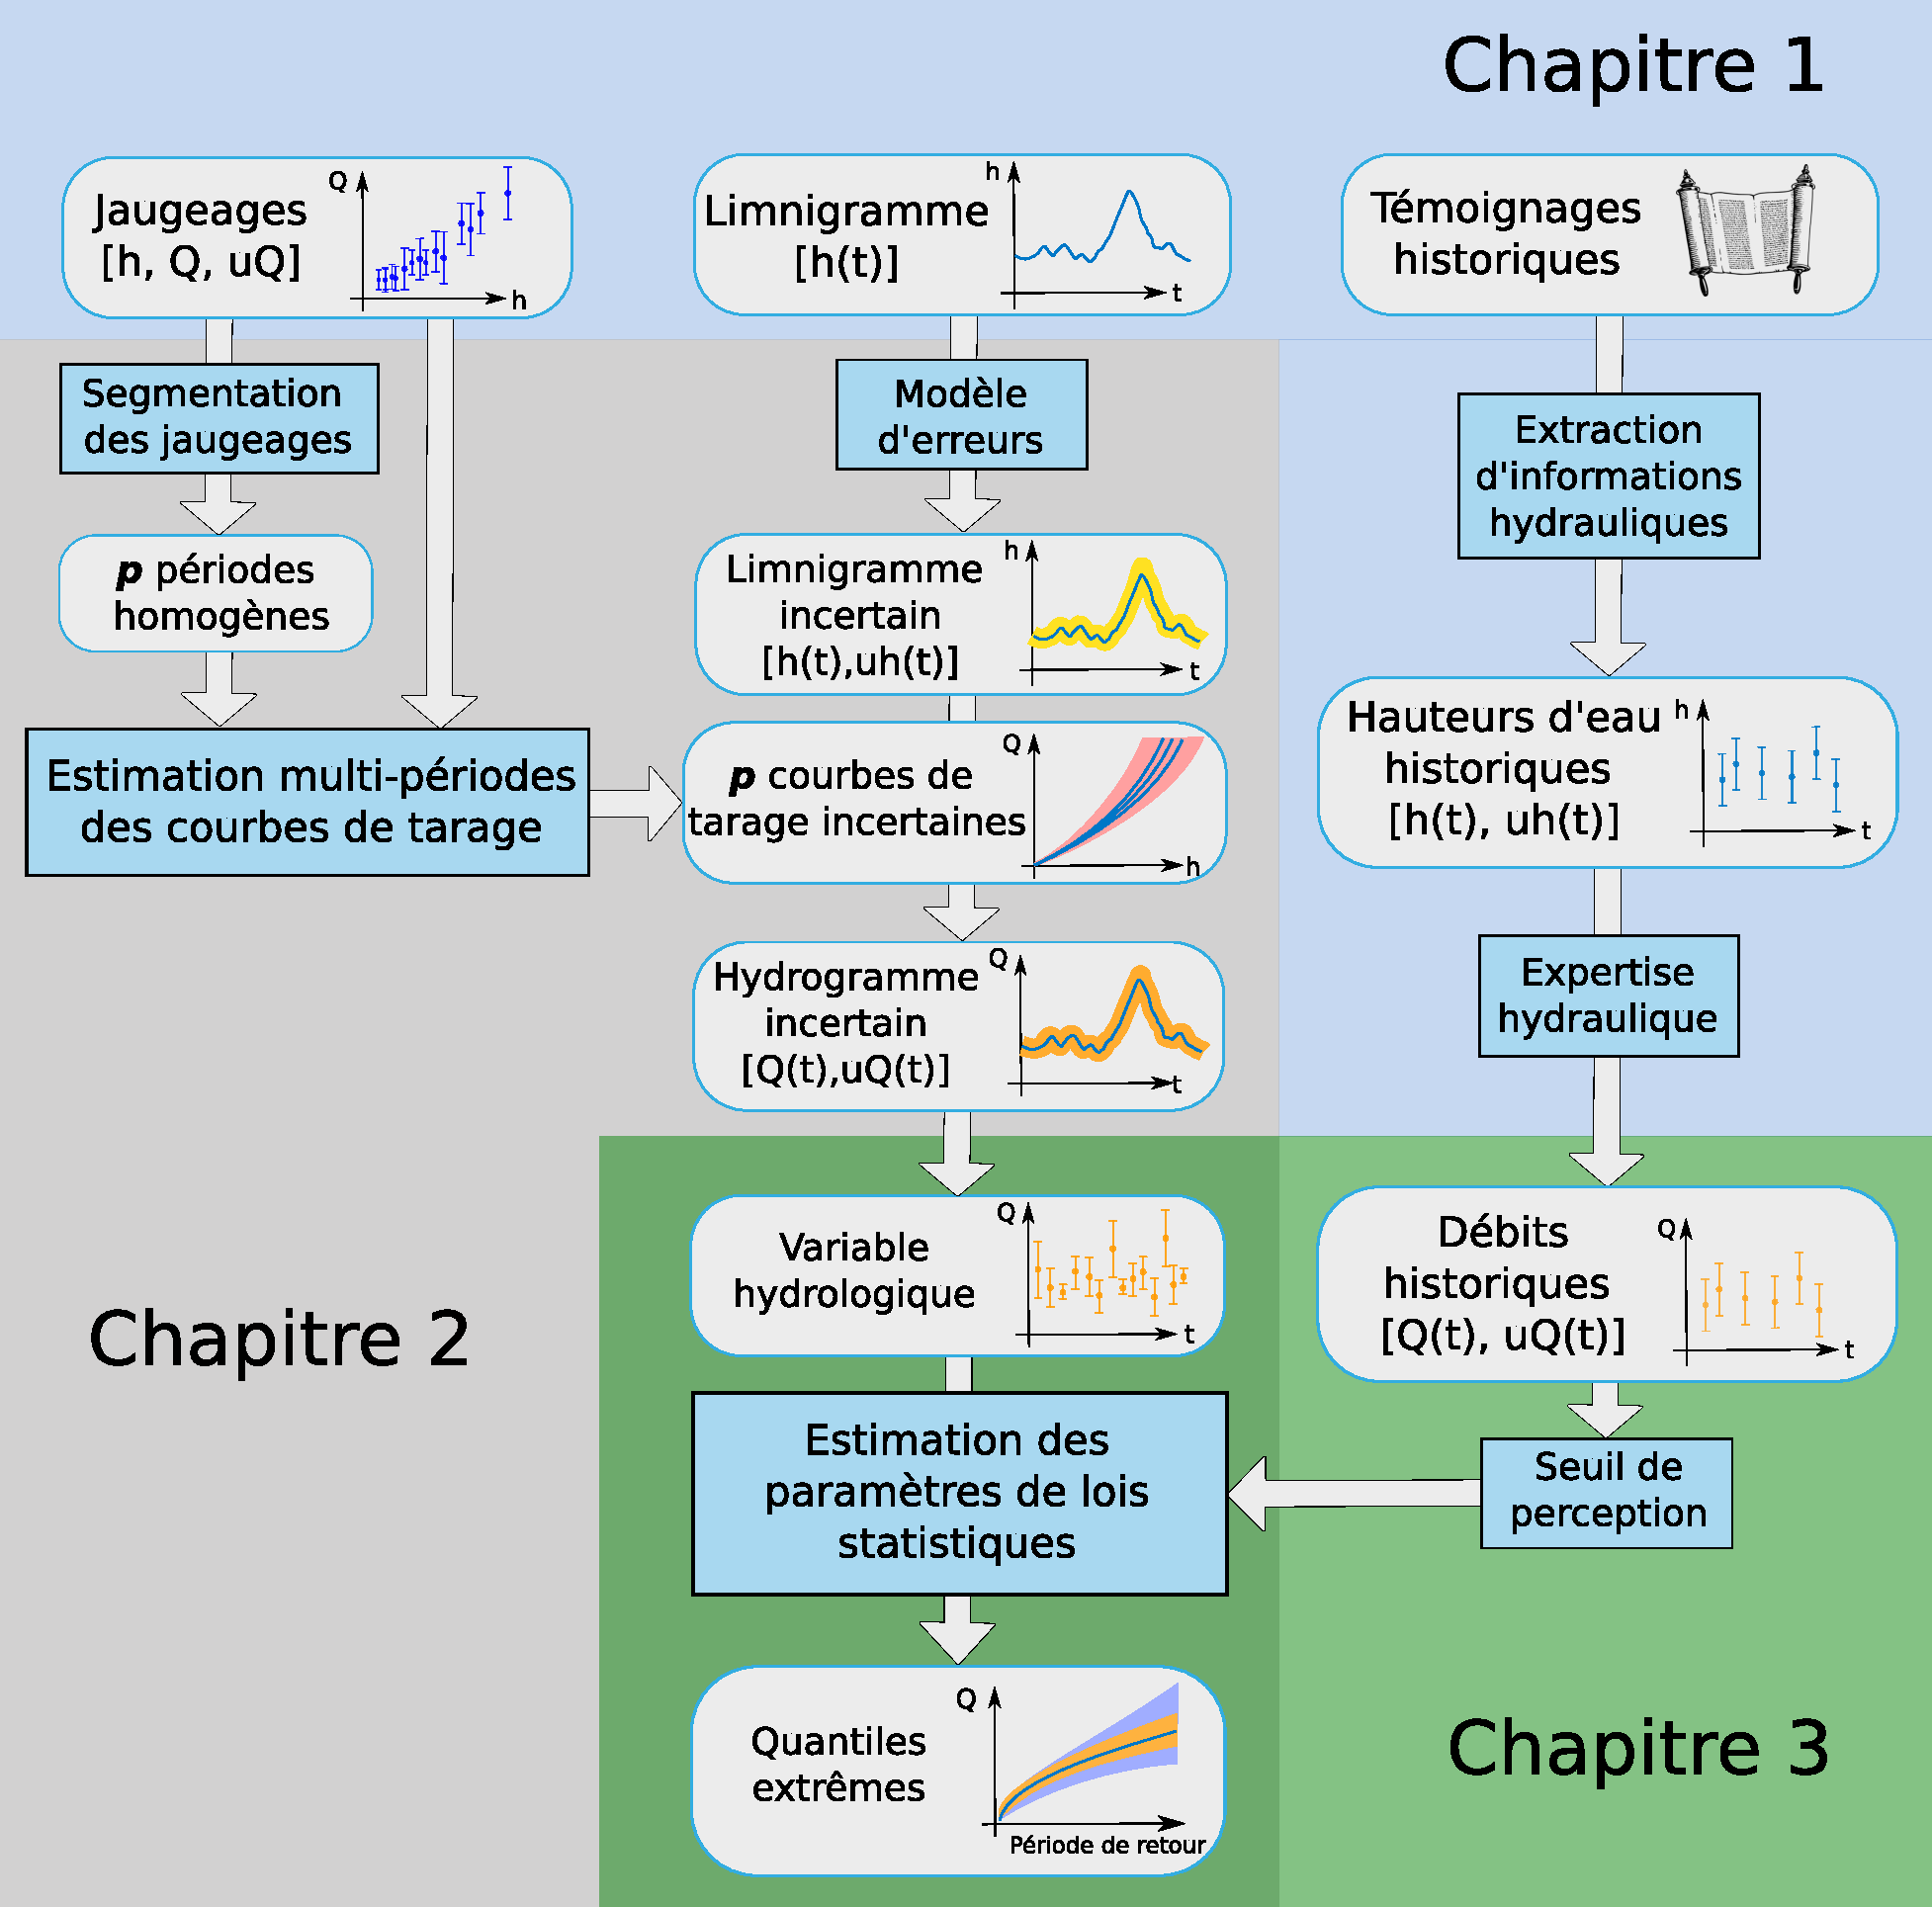
\includegraphics[width = .6\textwidth]{./Figures/SchemaThese.pdf} 
 	\end{frame}
	
\section{Le Rhône à Beaucaire}
	\subsection{Le Rhône à Beaucaire}
	{
    \setbeamercolor{background canvas}{bg=myblue}
    \begin{frame}
        \begin{center}
				\textcolor{white}{\Large \textbf{Le Rhône à Beaucaire}}\\
		 		\vspace{0.3cm}
		 		\textcolor{white}{\large \textbf{Collecte et caractérisation des données de crue}}\\
		 		\vspace{0.8cm}
		 		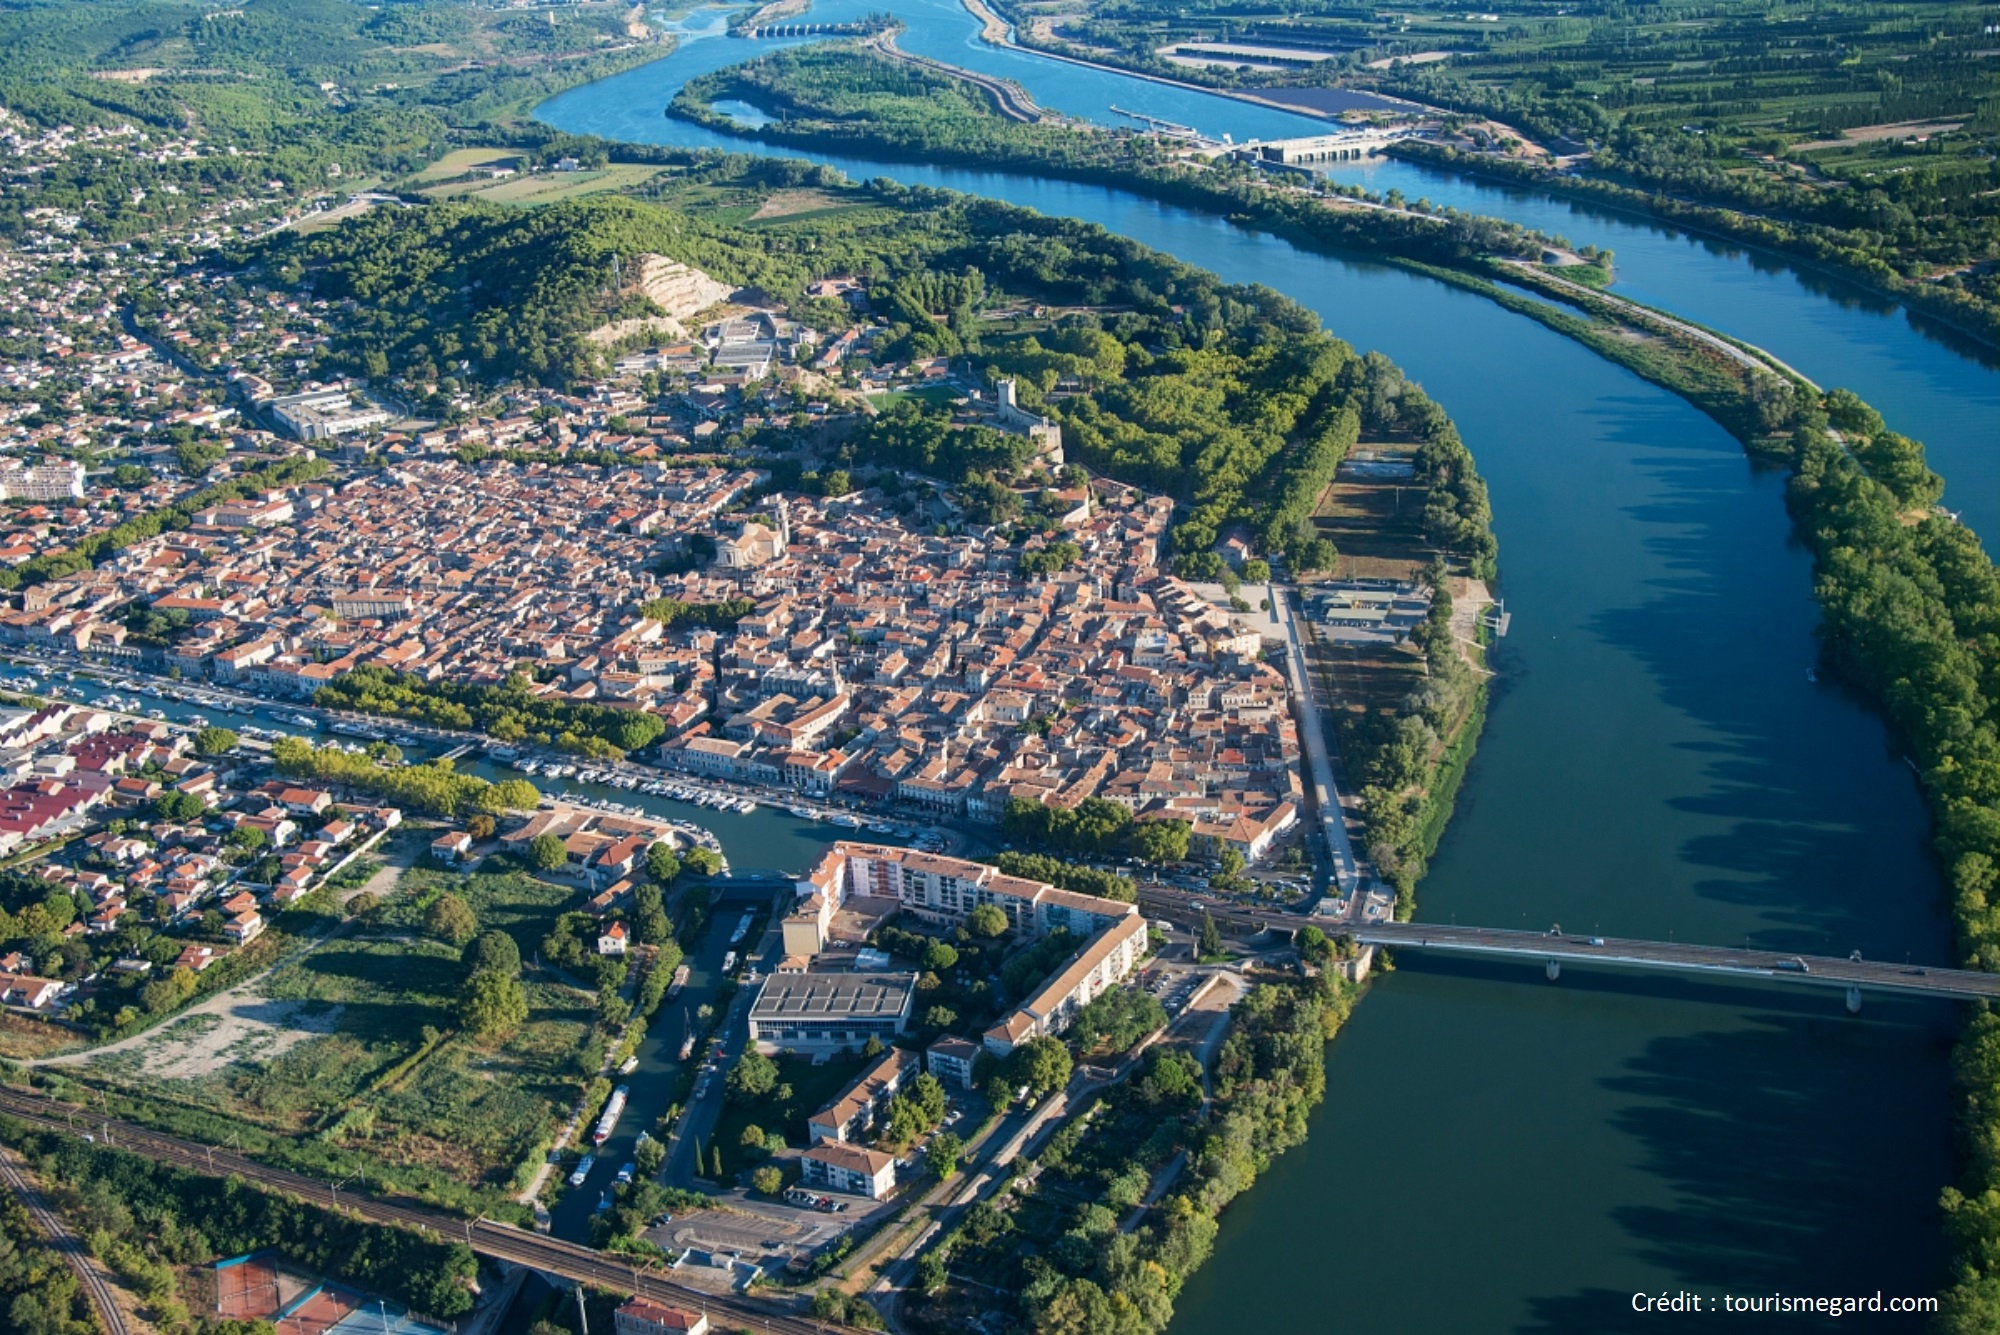
\includegraphics[width = .7\textwidth]{./Figures/BcrAerien.jpg} 
        \end{center}
    \end{frame}
    }
    	
    	\subsection{Station hydrométrique}
	%%%%%%%%% 19 %%%%%%%%%
	\begin{frame}%[c]
		\frametitle{Présentation de la station}
		\begin{minipage}{.55\textwidth}
			\begin{itemize}
				\item<1->[$\vartriangleright$] Bassin versant de 95 590 km²
				\vspace{5pt}
				\item<2->[$\vartriangleright$] Plus fort débit français
				\vspace{5pt}
				\item<3->[$\vartriangleright$] Apports variés et complexes : \og\textit{il comporte une infinité de nuances et de contrastes}\fg{}   \footfullcite{parde_regime_1925}
				\vspace{5pt}
				\item<4->[$\vartriangleright$] Dernière station du Rhône complet
			\end{itemize}
		\end{minipage}
		\begin{minipage}{.4\textwidth}
			\centering
	      	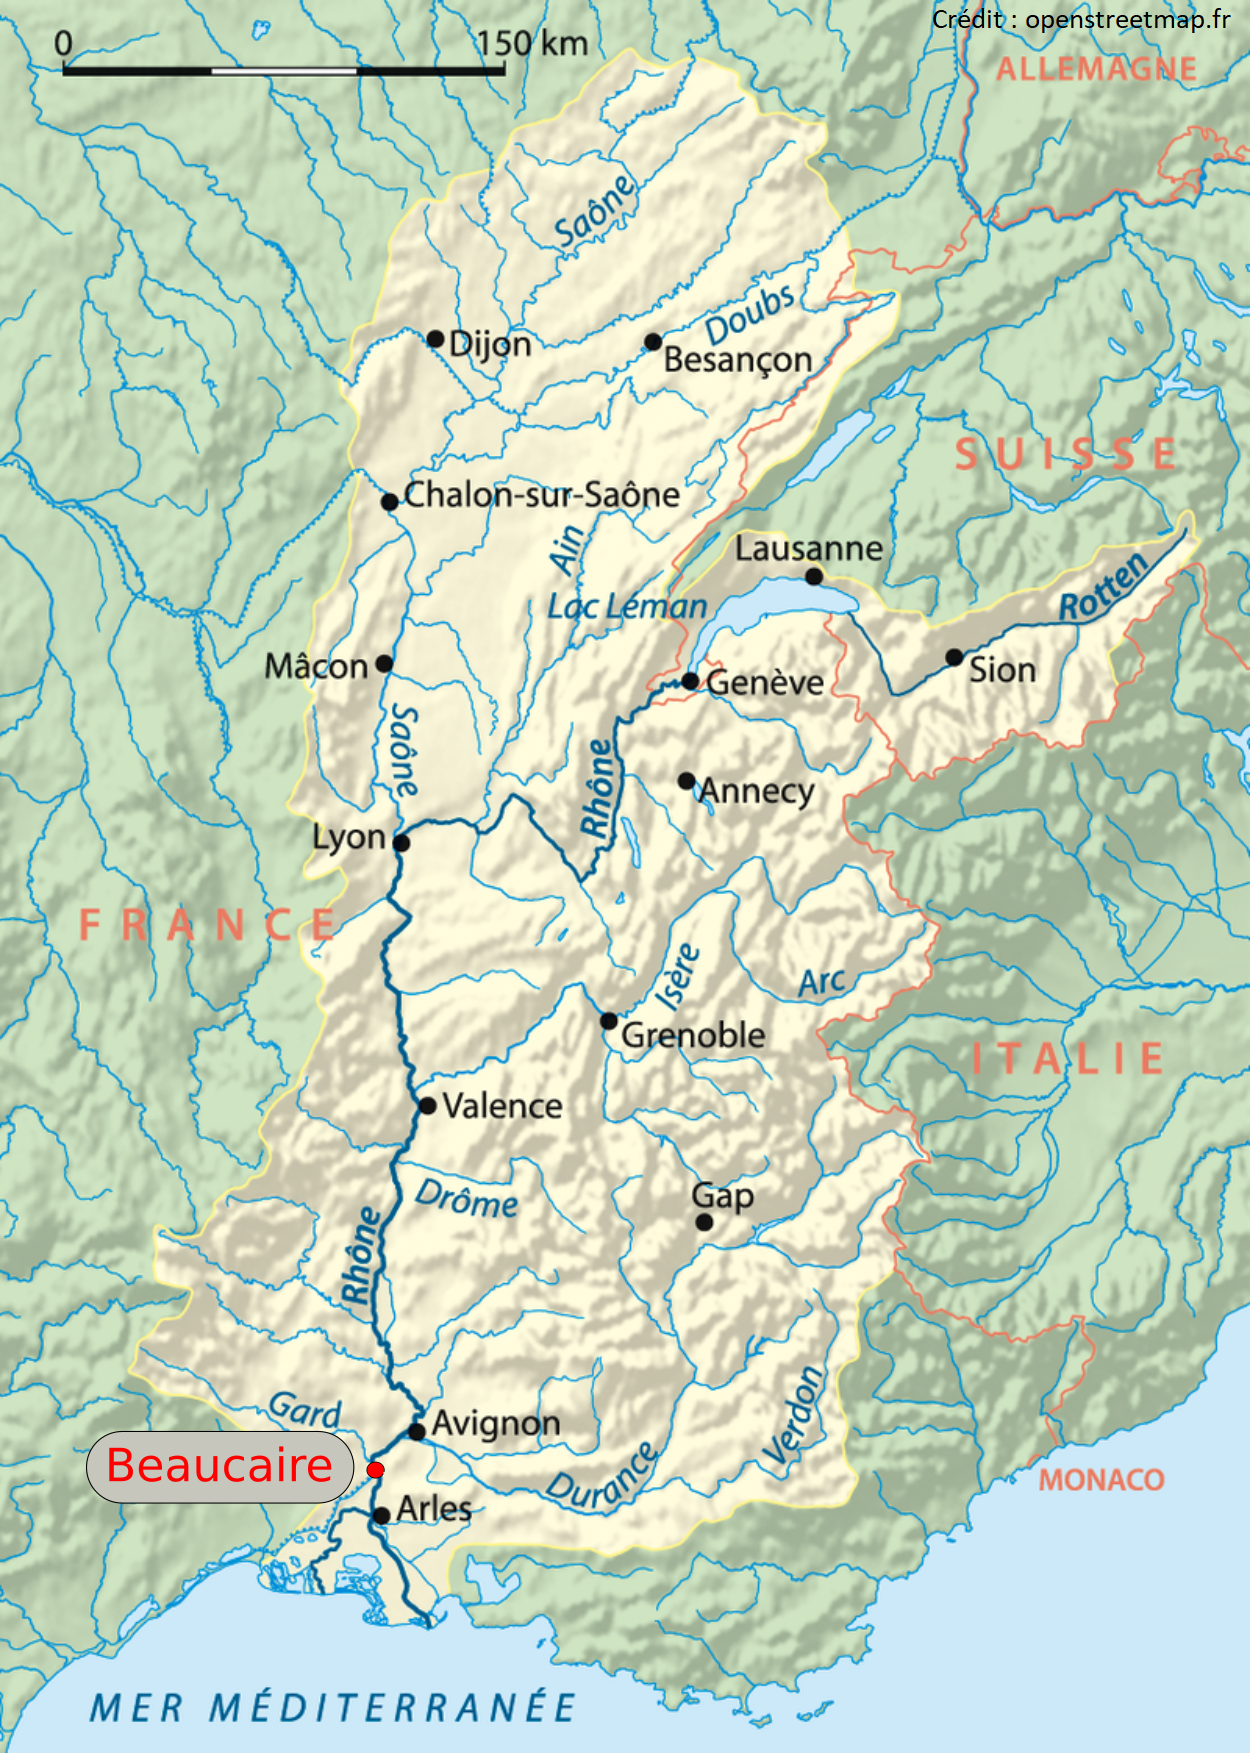
\includegraphics[width = \textwidth]{./Figures/Rhone_bassin_versant.png} 
		\end{minipage}
	\end{frame}
	
	%%%%%%%%% 20 %%%%%%%%%
	\begin{frame}%[c]
		\frametitle{Régime hydrologique}
		\centering
      	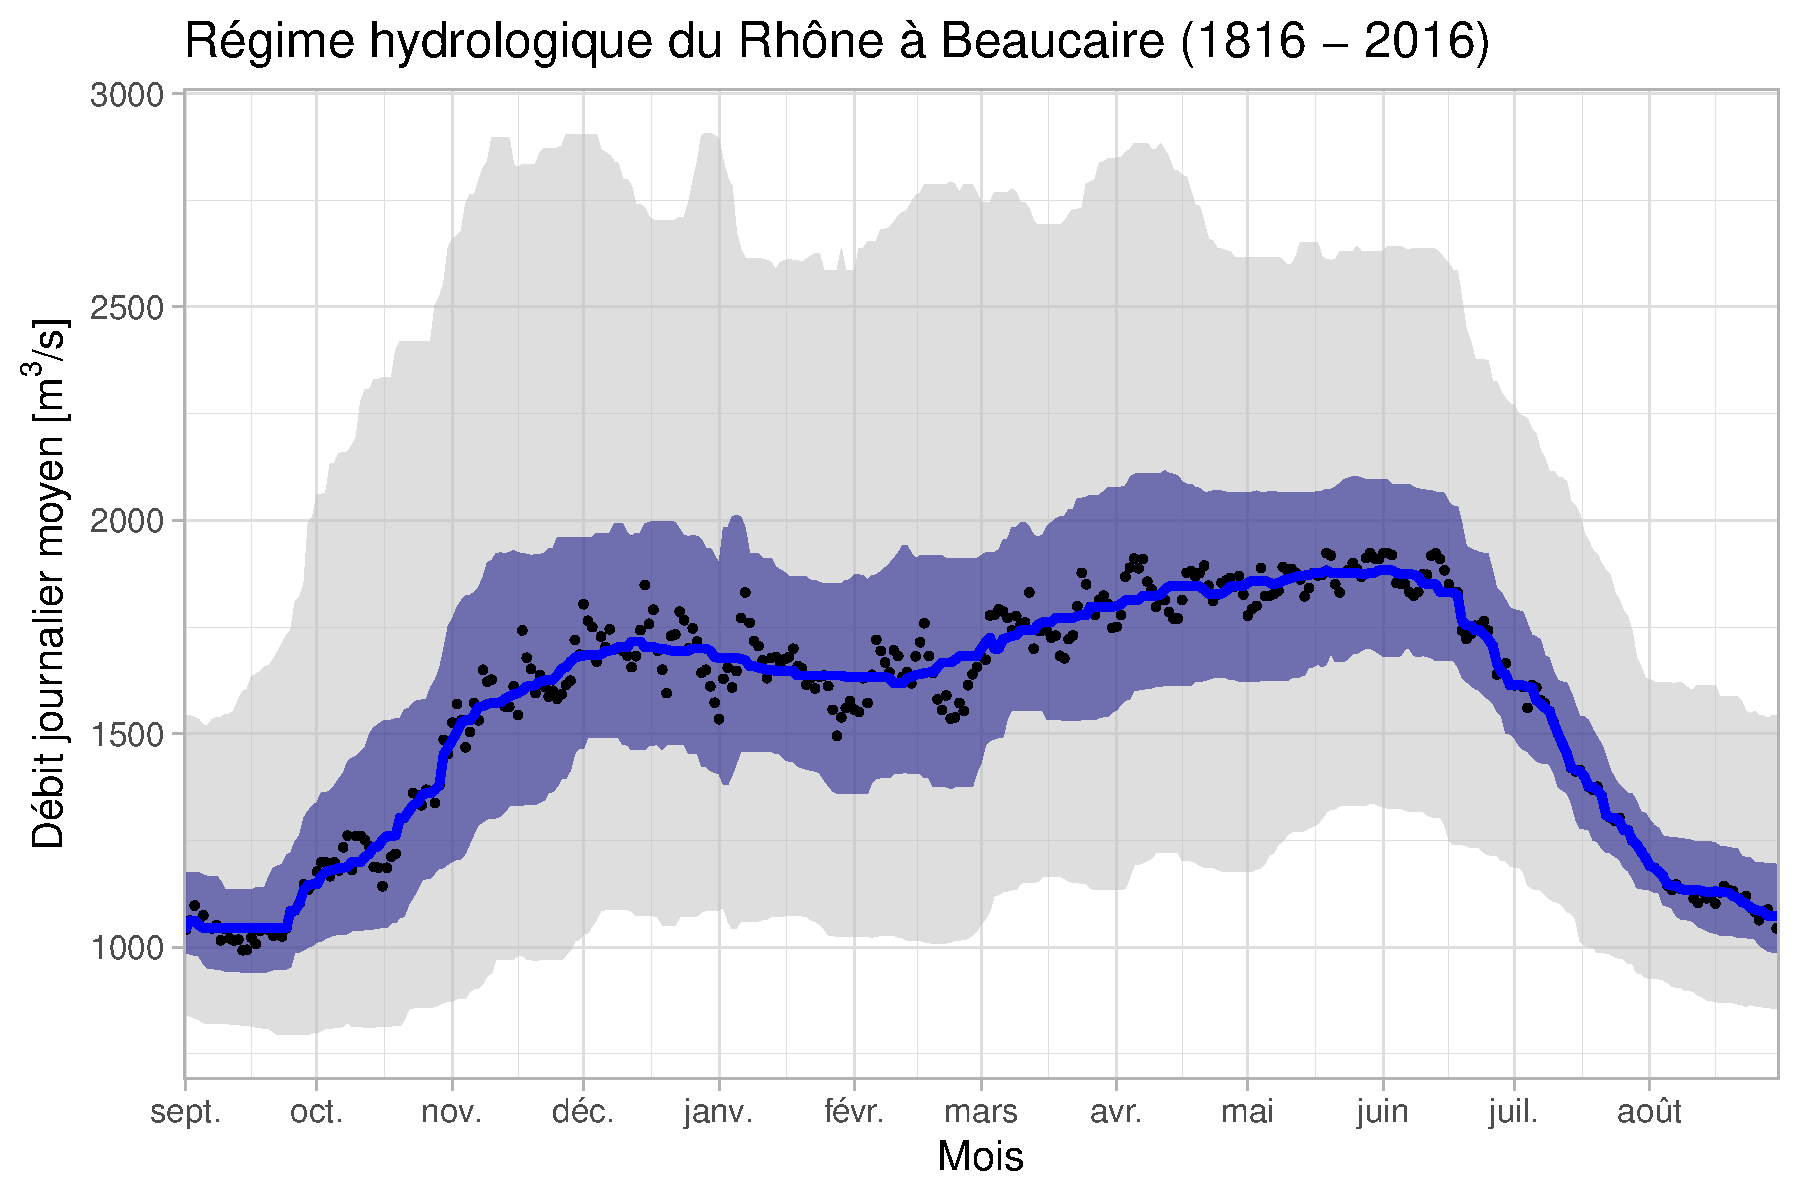
\includegraphics[width = .7\textwidth]{./Figures/Regime.pdf}\phantom{s}\\
      	\centering     	
      	Débits moyens journaliers et quantiles (20, 40, 60 et 80\%)
	\end{frame}
	
	%%%%%%%%% 21 %%%%%%%%%
	\begin{frame}%[c]
		\frametitle{Beaucaire et le Rhône}
		\begin{minipage}{.49\textwidth}
			\begin{itemize}
				\item<1->[$\vartriangleright$] Foire de Beaucaire : \og \textit{Capitale française des marchandises} \fg{}\footfullcite{leon_vie_1953}
				\vspace{5pt}
				\item<2->[$\vartriangleright$] Fortes crues au XIX\textsuperscript{ème} siècle
				\vspace{5pt}
				\item<3->[$\vartriangleright$] Début des relevés en 1816
				\vspace{5pt}
			\end{itemize}
		\end{minipage}
		\begin{minipage}{.49\textwidth}
			\begin{center}
	      		\includegraphics<1>[width = \textwidth]{./Figures/foire5.jpg} 
	      		\includegraphics<2>[width = \columnwidth]{./Figures/Napo.jpg} 
%	      		\includegraphics<3>[width = \columnwidth]{./Figures/Avi2003.jpg} 
	      		\includegraphics<3>[width = .6\textwidth]{./Figures/StationBcr.jpg} 
			\end{center}
		\end{minipage}
	\end{frame}
	
	%%%%%%%%% 22 %%%%%%%%%
	\begin{frame}%[c]
		\frametitle{Station hydrométrique (1816-2020)}
		\begin{minipage}{.45\textwidth}
			\begin{itemize}
				\item<1->[$\vartriangleright$] Relevés quotidiens dès 1816 : "\textbf{Pont de Beaucaire}"
				\vspace{2pt}
				\item<2->[$\vartriangleright$] Travaux CNR 1967-1970
				\vspace{2pt}
				\item<3->[$\vartriangleright$] Déplacement 2 km à l'aval : "\textbf{Beaucaire Restitution}"
				\vspace{2pt}
				\item<4->[$\vartriangleright$] 205 ans de relevés à Beaucaire
				\vspace{2pt}
				\item<5->[$\vartriangleright$] Jaugeages dès 1845
			\end{itemize}
		\end{minipage}
		\begin{minipage}{.53\textwidth}
			\begin{center}
	      		\includegraphics<1>[width = \textwidth]{./Figures/PtBcr.png} 
	      		\includegraphics<2>[width = \columnwidth]{./Figures/TabObs.jpg} 
	      		\includegraphics<3-4>[width = \columnwidth]{./Figures/BcrRestit.png} 
	      		\includegraphics<5>[width = \textwidth]{./Figures/Jaus.pdf}
			\end{center}
		\end{minipage}
	\end{frame}
	
 	\subsection{HISTRHÔNE (1300-2000)}
	%%%%%%%%% 23 %%%%%%%%%
	\begin{frame}%[c]
		\frametitle{Base de données HISTRHÔNE (1300-2000)}
\begin{minipage}{.45\textwidth}
			\begin{itemize}
				\item<1->[$\vartriangleright$] Base de données d'événements hydroclimatiques en basse vallée du Rhône \footfullcite{pichard_sept_2014}
				\vspace{2pt}
				\item<2->[$\vartriangleright$] 1500 événements du XIII\textsuperscript{ème} siècle à 2000
				\vspace{2pt}
				\item<3->[$\vartriangleright$] Classés par type et par gravité 
			\end{itemize}
		\end{minipage}
		\begin{minipage}{.54\textwidth}
			\begin{center}
	      		\includegraphics<1-2>[width = .75\textwidth]{./Figures/HistrhoneMap.jpg} 
	      		\includegraphics<3>[width = .75\columnwidth]{./Figures/CatHistrhone.png}\phantom{s}\\
				\vspace{1pt}				
				\tiny{Tiré de \url{histrhone.cerege.fr}} 
			\end{center}
		\end{minipage}
	\end{frame}
	
	
\section{1816-2020}
	\subsection{Chaine de propagation}
	{
    \setbeamercolor{background canvas}{bg=myblue}
    \begin{frame}
        \begin{center}
%				\textcolor{white}{\Large \textbf{1816-2020}}\\
%		 		\vspace{0.3cm}
		 		\textcolor{white}{\Large \textbf{Chaine de propagation des incertitudes}}\\
		 		\vspace{1cm}
		 		\textcolor{white}{\large \textbf{Valoriser les données hydrométriques disponibles\\
		 		 depuis 1816 à Beaucaire}}\\
        \end{center}
    \end{frame}
    }
    
    %%%%%%%%% 25 %%%%%%%%%
    \begin{frame}
    		\frametitle{Chaine de propagation des incertitudes}
    		\begin{center}
      		\includegraphics<1>[width = .44\textwidth]{./Figures/SchemaProp1.pdf} 
			\includegraphics<2>[width = .44\textwidth]{./Figures/SchemaProp2.pdf} 
			\includegraphics<3>[width = .44\textwidth]{./Figures/SchemaProp3.pdf} 
			\includegraphics<4>[width = .44\textwidth]{./Figures/SchemaProp0.pdf} 	
	     \end{center}
    \end{frame}
	
	\subsection{Segmentation des jaugeages}
	%%%%%%%%% 26 %%%%%%%%%
    \begin{frame}
    	\frametitle{Segmentation des jaugeages}
		\begin{minipage}{.35\textwidth}
			\begin{itemize}
			\item<1->[$\vartriangleright$] Relation h/Q régulièrement perturbée
			\vspace{0.5cm}
			\item<2->[$\vartriangleright$] Courbe de tarage à revoir 
			\vspace{0.5cm}
			\item<3->[$\vartriangleright$] Détection des ruptures \footfullcite{darienzo_detection_2021}\\
						\end{itemize}
		\end{minipage}
		\begin{minipage}{.6\textwidth}
			\begin{center}
				\includegraphics<1-2>[width = .8\textwidth]{./Figures/Vesubie.jpg} 
				\includegraphics<3>[width = .7\textwidth]{./Figures/Matt.jpg} 	
				\includegraphics<4>[width = \textwidth]{./Figures/SegmPt.pdf} 		
			\end{center}
		\end{minipage}
    \end{frame}
    
    \subsection{CT}
    %%%%%%%%% 27 %%%%%%%%%
\begin{frame}
    	\frametitle{Estimation des courbes de tarage}
		\begin{minipage}{.4\textwidth}
		\begin{itemize}
			\item<1->[$\vartriangleright$] Définition des contrôles hydrauliques
			\vspace{0.5cm}
			\item<2->[$\vartriangleright$] Équation de courbe de tarage  
			\vspace{0.5cm}
			\item<3->[$\vartriangleright$] Estimation bayésienne des courbes \footfullcite{le_coz_combining_2014}
			\vspace{0.5cm}
			\item<4->[$\vartriangleright$] Prise en compte de l'incertitude des jaugeages\\
						\end{itemize}
		\end{minipage}
		\begin{minipage}{.55\textwidth}
			\begin{center}
				\includegraphics<1>[width = \textwidth]{./Figures/Controles.jpg} 
				\onslide<2-> $Q = a(h-b)^c$\\
				\vspace{0.5cm}
				\includegraphics<3->[width = .9\textwidth]{./Figures/EqBaratin.jpg}
			\end{center}
		\end{minipage}
    \end{frame}
    
    %%%%%%%%% 28 %%%%%%%%%
    \begin{frame}
    	\frametitle{Estimation des courbes de tarage}
		\begin{minipage}{.44\textwidth}
		\begin{itemize}
			\item<1->[$\vartriangleright$] Périodes avec peu/pas de jaugeages ?
			\vspace{0.5cm}
			\item<2->[$\vartriangleright$] Paramètres constants entre périodes ? $\rightarrow$ expertise terrain
			\vspace{0.5cm}
			\item<3->[$\vartriangleright$] Modèle de courbes multipériodes\footfullcite{mansanarez_shift_2019}
			\vspace{0.5cm}
			\item<4->[$\vartriangleright$] Transfert d'informations entre périodes
			\vspace{0.5cm}
			\item<5->[$\vartriangleright$] Pas de "recyclage"
			\end{itemize}
			
		\end{minipage}
		\begin{minipage}{.55\textwidth}
			\begin{center}
				\includegraphics<1>[width = \textwidth]{./Figures/SegmPt.pdf} 
				\onslide<2> $Q = \textcolor{red}{a}(h-b)^{\textcolor{red}{c}}$	
				\includegraphics<3>[width = \textwidth]{./Figures/Spd.jpg} 	
				\includegraphics<4->[width = \textwidth]{./Figures/RClog_ICdownPt.pdf}  			
			\end{center}
		\end{minipage}    	   	
    \end{frame}
    
    \subsection{ulimni}
    %%%%%%%%% 29 %%%%%%%%%
    \begin{frame}
    		\frametitle{Incertitude limnimétrique}
		présentation 5 erreurs additives + calcul interpolation temporelle
		\includegraphics<1->[width = .8\textwidth]{./Figures/8-StageErrorAMAX_BOTH.pdf}  	
    \end{frame}
    
    %%%%%%%%% 30 %%%%%%%%%
    \begin{frame}
    		\frametitle{Hydrogramme 1816-2020}
		Plus long hydrogramme de France ? 
		\includegraphics<1->[width = .8\textwidth]{./Figures/9-IcAndAMAX.pdf}  	
    \end{frame}
    
    \subsection{GEV}
    %%%%%%%%% 31 %%%%%%%%%
    \begin{frame}
    		\frametitle{Estimation des débits caractéristiques}
		Schema explication de la propagation successive des 2 types d'incertitude	
    \end{frame}
    
     %%%%%%%%% 32 %%%%%%%%%
    \begin{frame}
    		\frametitle{Estimation des débits caractéristiques}
		\includegraphics<1->[width = .8\textwidth]{./Figures/10a-GeV_205years.pdf}  
    \end{frame}
   
    %%%%%%%%% 33 %%%%%%%%%
    \begin{frame}
    		\frametitle{Sensibilité à la taille d'échantillon}
		\includegraphics<1->[width = .8\textwidth]{./Figures/10e-Q1000SSize.pdf}  
    \end{frame}

\section{1500-2020}
	\subsection{aa}
	{
    \setbeamercolor{background canvas}{bg=myblue}
    \begin{frame}
        \begin{center}
				\textcolor{white}{\Large \textbf{1500-2020}}\\
		 		\vspace{0.3cm}
		 		\textcolor{white}{\large \textbf{aaae}}\\
		 		\vspace{1cm}
%		 		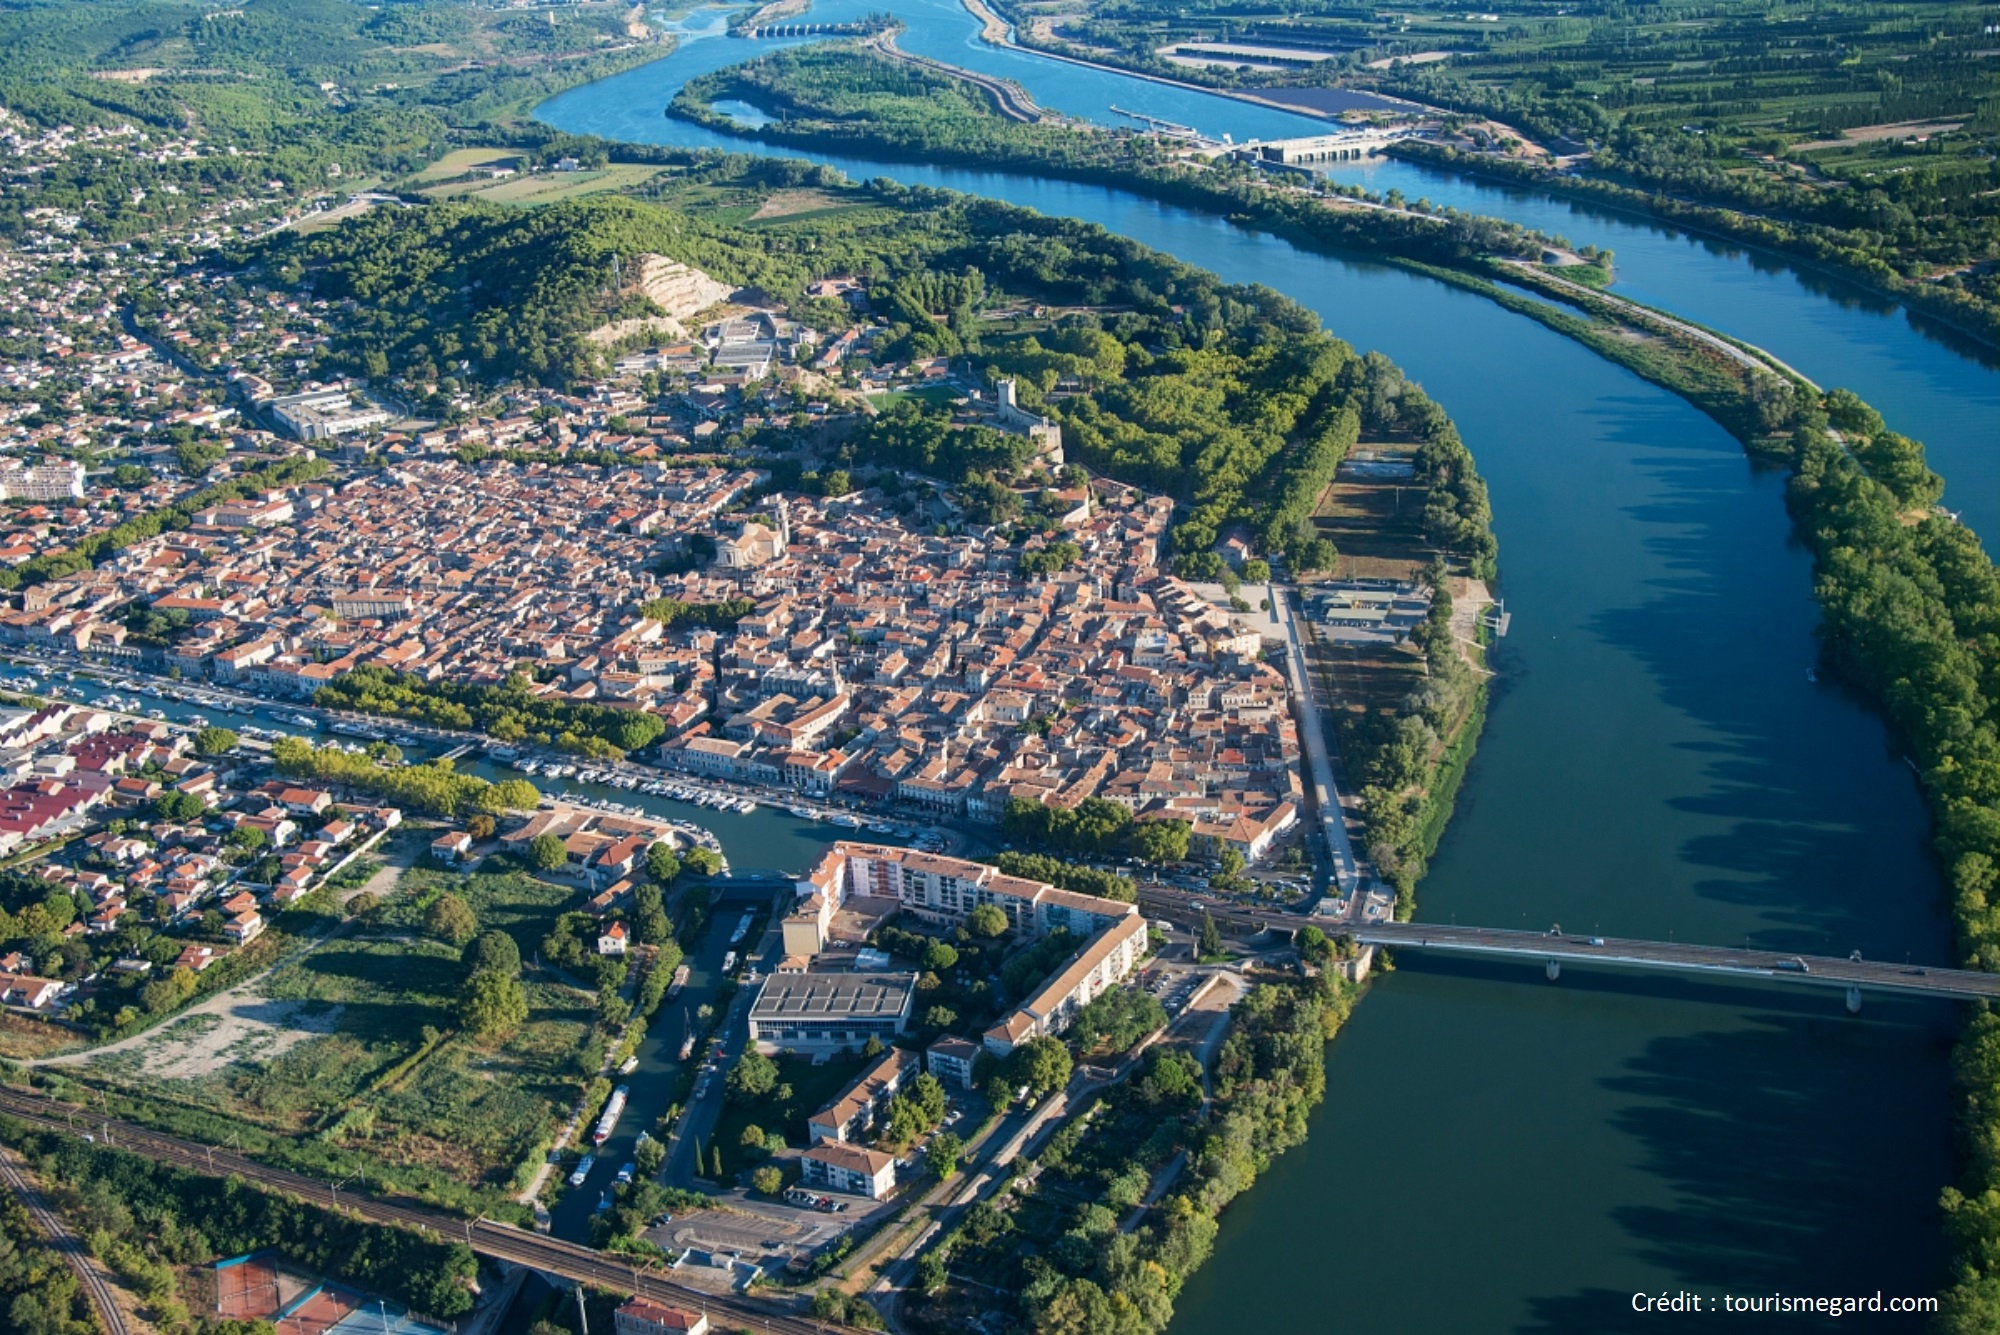
\includegraphics[width = .7\textwidth]{./Figures/BcrAerien.jpg} 
        \end{center}
    \end{frame}
    }
	\subsection{Donnes histo}
	%%%%%%%%% 35 %%%%%%%%%
    \begin{frame}
    		\frametitle{Données dispo}
    		explication evolution perception C3/C4 + échec modélisation 
	\end{frame}
	
	%%%%%%%%% 36 %%%%%%%%%
    \begin{frame}
    		\frametitle{Seuil de perception}
    		concept seuil de perception + nombre de dépassements + date de début \cite{stedinger_flood_1986}
	\end{frame}
	
    \subsection{Modèles}
    	%%%%%%%%% 37 %%%%%%%%%
    \begin{frame}
    		\frametitle{Modèle fréquentiel}
    		Equation vraisemblance avec parties en couleur + explication 4 modèles
	\end{frame}
	
	\subsection{Degradée}
	%%%%%%%%% 38 %%%%%%%%%
    \begin{frame}
    		\frametitle{Chronique dégradée (1816-2020)}
    		Résultats chronique dégradée + explication réduction incertitude VS baseline
	\end{frame}
	
	%%%%%%%%% 39 %%%%%%%%%
    \begin{frame}
    		\frametitle{Chronique dégradée (1816-2020)}
    		QUID SI Q connu ? modèle E
	\end{frame}
	\subsection{Complète}
	%%%%%%%%% 40 %%%%%%%%%
    \begin{frame}
    		\frametitle{Chronique complète (1500-2020)}
    		Résultats chronique complète + explication non-exhaustivité
	\end{frame}
    
\section{Conclusion}
	\subsection{Conclusion}
	{
    \setbeamercolor{background canvas}{bg=myblue}
    \begin{frame}
        \begin{center}
				\textcolor{white}{\Large \textbf{Conclusion}}\\
		 		\vspace{0.3cm}
%		 		\textcolor{white}{\large \textbf{Collecte et caractérisation des données de crue}}\\
%		 		\vspace{1cm}
%		 		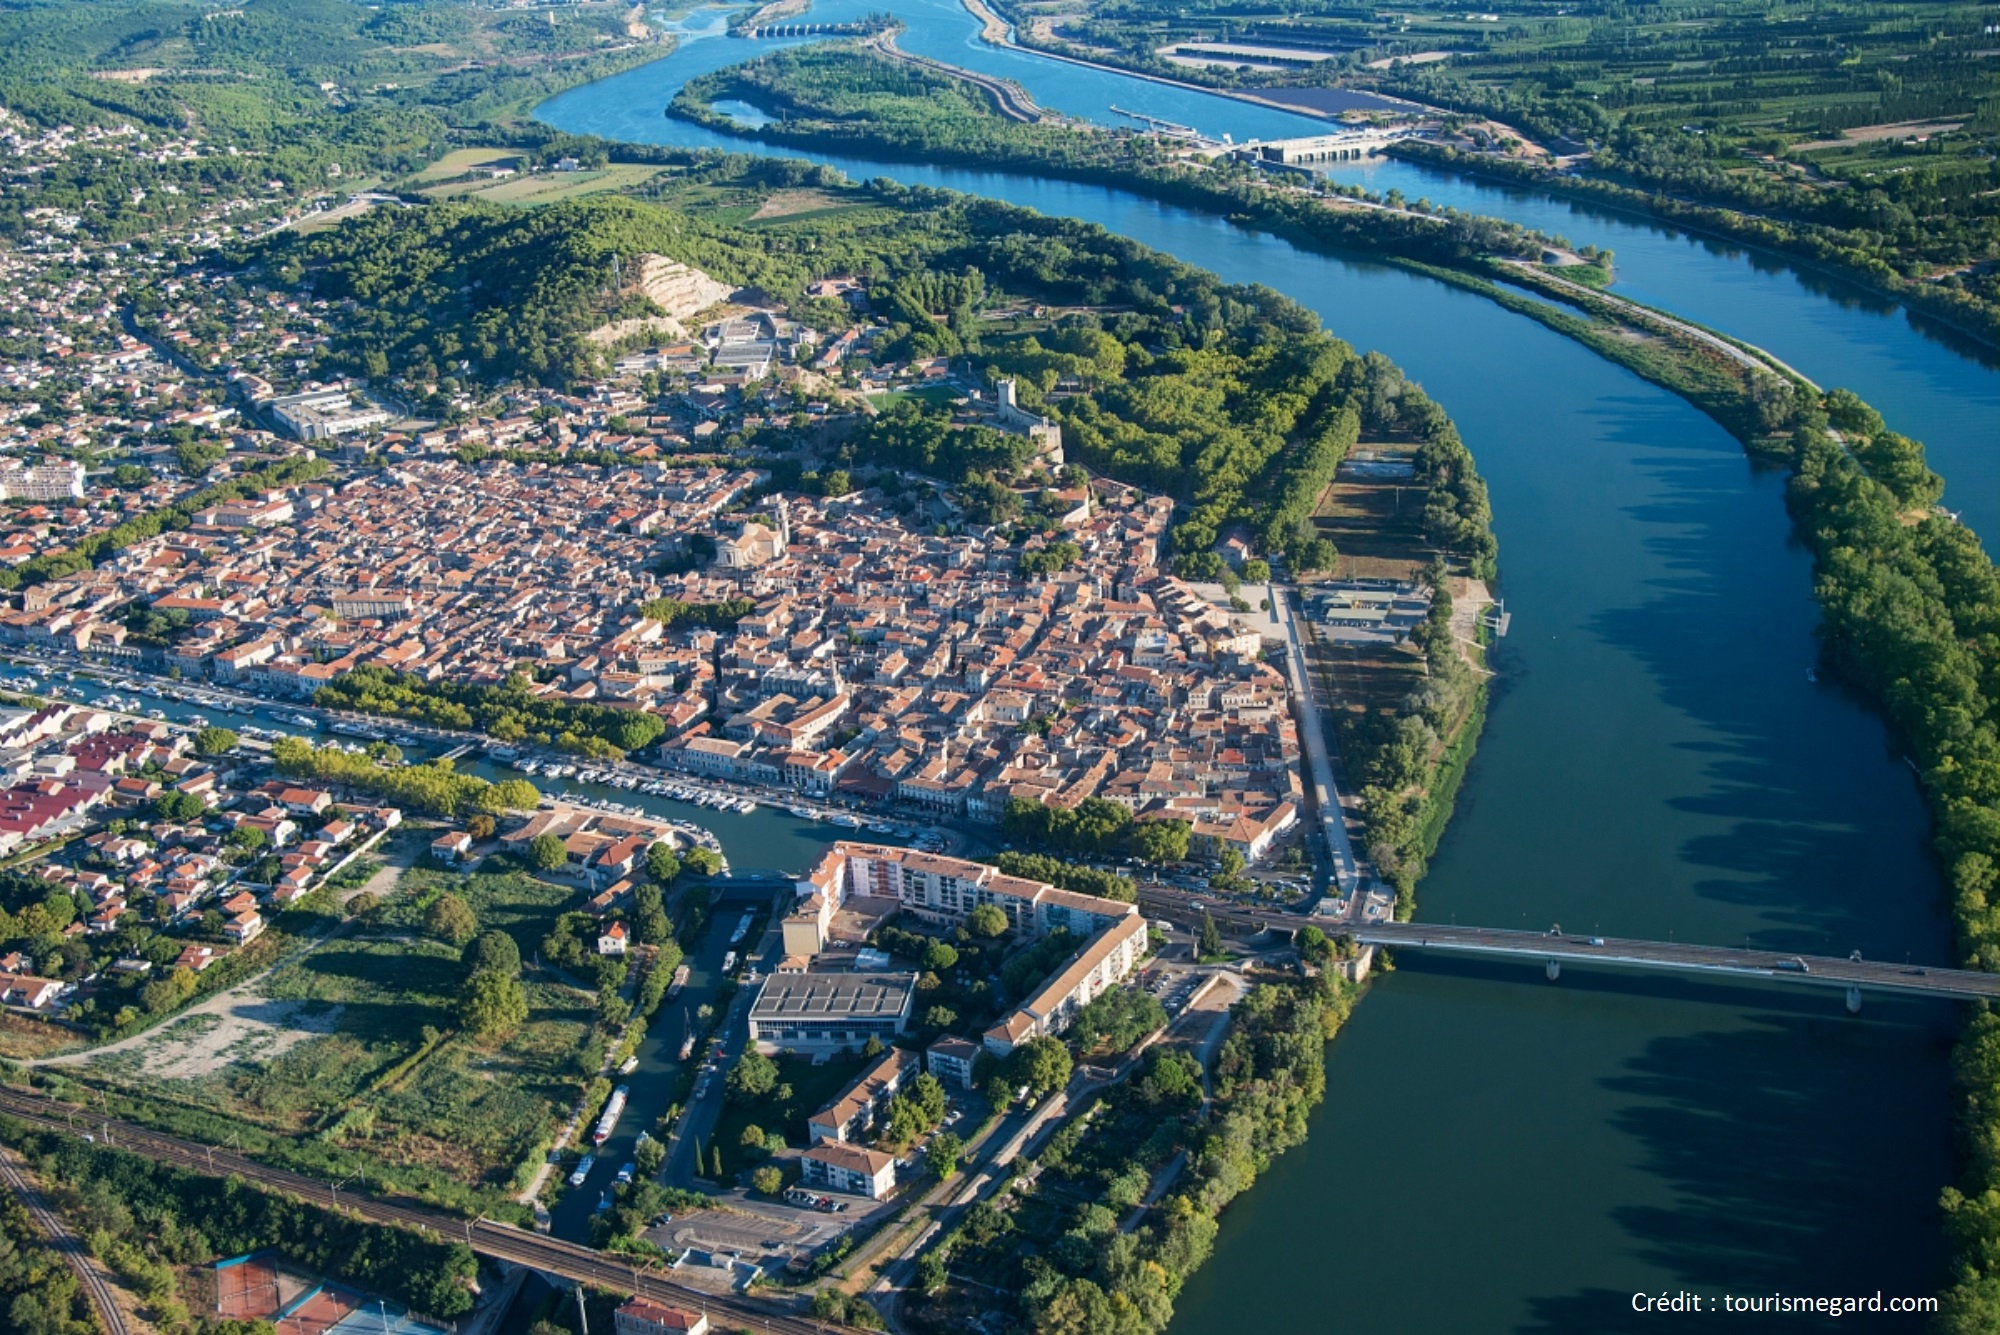
\includegraphics[width = .7\textwidth]{./Figures/BcrAerien.jpg} 
        \end{center}
    \end{frame}
    }
    
	\subsection{Limites}
	\subsection{Perspectives}
	\subsection{Remerciements}
	
%\printbibliography
	
\section{Annexes}
%slide tests homogénéité
%slides modélisation hydraulique
%slides réponses reviewers



%\begin{frame}
%	\printbibliography
%\end{frame}





\end{document}
